% Standalone TikZ: Attitude Adjustment 3D Isometric  
% Left = tilted body with p_raw, Right = leveled body with p_adj
\documentclass[border=10pt]{standalone}
\usepackage[utf8]{inputenc}
\usepackage[T5]{fontenc}
\usepackage{tikz}
\usepackage{amsmath,amssymb,bm}
\usetikzlibrary{arrows.meta,calc}

\begin{document}
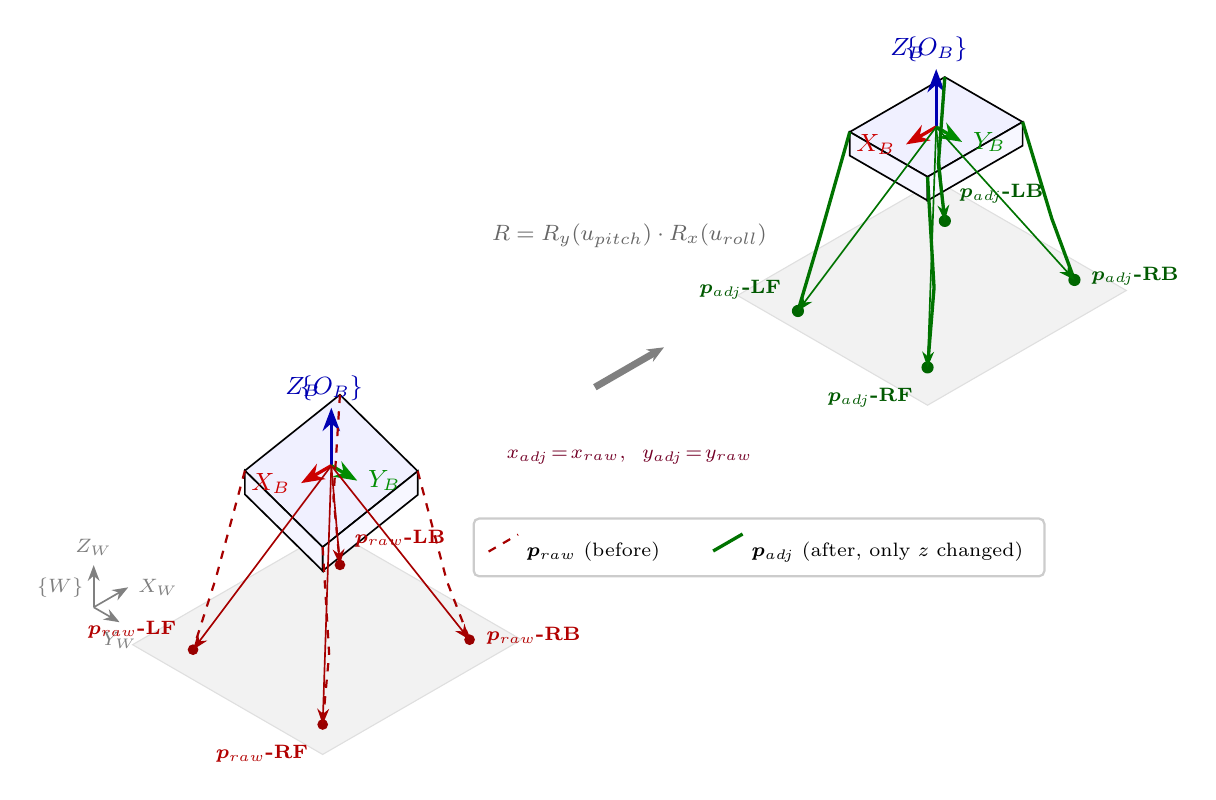
\begin{tikzpicture}[
    >=Stealth,
    scale=0.88,
    x={({cos(30)*0.72cm},{sin(30)*0.72cm})},
    y={({-cos(30)*0.72cm},{sin(30)*0.72cm})},
    z={(0cm,0.76cm)},
    thick,
]

% =============================================
%  World frame (top-left corner, isolated)
% =============================================
\coordinate (Wo) at (-8.5, 3.5, 0);
\draw[->, semithick, black!50] (Wo) -- ++(0.8,0,0) node[right, font=\scriptsize] {$X_W$};
\draw[->, semithick, black!50] (Wo) -- ++(0,-0.6,0) node[below, font=\scriptsize] {$Y_W$};
\draw[->, semithick, black!50] (Wo) -- ++(0,0,0.8) node[above, font=\scriptsize] {$Z_W$};
\node[font=\scriptsize\bfseries, black!50, above left] at (Wo) {$\{W\}$};

% =============================================
%  LEFT SIDE -- Tilted body, p_raw
% =============================================
\begin{scope}[shift={(-6.5,0,0)}]

    % Ground 
    \fill[gray!10, draw=gray!25, thin]
        (-2.3,-2.1,0) -- (2.3,-2.1,0) -- (2.3,2.3,0) -- (-2.3,2.3,0) -- cycle;
    
    % Body box (tilted: back-left high, front-right low)
    \coordinate (A1) at (-1.1, 0.9, 3.4);
    \coordinate (A2) at (-1.1,-0.9, 2.8);
    \coordinate (A3) at ( 1.1,-0.9, 3.2);
    \coordinate (A4) at ( 1.1, 0.9, 3.8);
    \fill[blue!6, draw=black, semithick] (A1)--(A2)--(A3)--(A4)--cycle;
    \fill[blue!4, draw=black, semithick] (A1)--(A2)--($(A2)+(0,0,-0.45)$)--($(A1)+(0,0,-0.45)$)--cycle;
    \fill[blue!3, draw=black, semithick] (A2)--(A3)--($(A3)+(0,0,-0.45)$)--($(A2)+(0,0,-0.45)$)--cycle;

    % Body frame
    \coordinate (C1) at (0,0,3.4);
    \draw[->, very thick, blue!70!black] (C1) -- ++(0,0,1.1)
        node[above left, font=\small\bfseries] {$Z_B$};
    \draw[->, very thick, red!80!black]  (C1) -- ++(-0.7,0,0)
        node[left, font=\small\bfseries] {$X_B$};
    \draw[->, very thick, green!55!black] (C1) -- ++(0,-0.6,0)
        node[right, font=\small\bfseries] {$Y_B$};
    \node[blue!70!black, font=\small\bfseries] at ($(C1)+(0.5,0.5,1.0)$) {$\{O_B\}$};

    % Feet
    \coordinate (fLF) at (-1.7, 1.5, 0);
    \coordinate (fRF) at (-1.7,-1.5, 0);
    \coordinate (fLB) at ( 1.7, 1.5, 0);
    \coordinate (fRB) at ( 1.7,-1.5, 0);

    % Legs (two-segment, dashed red)
    \draw[red!65!black, thick, dashed]
        (A1) -- ($(A1)!0.52!(fLF)+(0.05,0.1,-0.35)$) -- (fLF);
    \draw[red!65!black, thick, dashed]
        (A2) -- ($(A2)!0.52!(fRF)+(0.05,-0.1,-0.25)$) -- (fRF);
    \draw[red!65!black, thick, dashed]
        (A4) -- ($(A4)!0.52!(fLB)+(-0.05,0.1,-0.3)$) -- (fLB);
    \draw[red!65!black, thick, dashed]
        (A3) -- ($(A3)!0.52!(fRB)+(-0.05,-0.1,-0.35)$) -- (fRB);

    % Foot dots
    \foreach \p in {fLF,fRF,fLB,fRB}
        \fill[red!60!black] (\p) circle[radius=2.2pt];

    % Vector arrows from body center to feet
    \draw[->, red!65!black, semithick] (C1) -- (fLF);
    \draw[->, red!65!black, semithick] (C1) -- (fRF);
    \draw[->, red!65!black, semithick] (C1) -- (fLB);
    \draw[->, red!65!black, semithick] (C1) -- (fRB);

    % Labels
    \node[red!70!black, font=\scriptsize\bfseries, above left]  at ($(fLF)+(-0.15,0,0.1)$) 
        {$\bm{p}_{raw}$-LF};
    \node[red!70!black, font=\scriptsize\bfseries, below left]  at ($(fRF)+(-0.1,0,-0.15)$) 
        {$\bm{p}_{raw}$-RF};
    \node[red!70!black, font=\scriptsize\bfseries, above right] at ($(fLB)+(0.1,0,0.1)$) 
        {$\bm{p}_{raw}$-LB};
    \node[red!70!black, font=\scriptsize\bfseries, right]       at ($(fRB)+(0.15,0,0)$) 
        {$\bm{p}_{raw}$-RB};
\end{scope}

% =============================================
%  TRANSITION ARROW  (middle, isolated)
% =============================================
\draw[-{Stealth[length=6pt,width=5pt]}, line width=2.5pt, black!50]
    (-0.4, 0, 2.0) -- (1.2, 0, 2.0);

\node[font=\footnotesize\bfseries, text=black!60, align=center] at (0.4, 0, 4.5)
    {$R = R_y(u_{pitch}) \cdot R_x(u_{roll})$};

\node[font=\scriptsize, text=purple!60!black] at (0.4, 0, 0.3)
    {$x_{adj}\!=\!x_{raw},\;\; y_{adj}\!=\!y_{raw}$};

% =============================================
%  RIGHT SIDE -- Leveled body, p_adj
% =============================================
\begin{scope}[shift={(7.5,0,0)}]

    % Ground
    \fill[gray!10, draw=gray!25, thin]
        (-2.3,-2.1,0) -- (2.3,-2.1,0) -- (2.3,2.3,0) -- (-2.3,2.3,0) -- cycle;

    % Body box (level)
    \coordinate (B1) at (-1.1, 0.9, 3.2);
    \coordinate (B2) at (-1.1,-0.9, 3.2);
    \coordinate (B3) at ( 1.1,-0.9, 3.2);
    \coordinate (B4) at ( 1.1, 0.9, 3.2);
    \fill[blue!6, draw=black, semithick] (B1)--(B2)--(B3)--(B4)--cycle;
    \fill[blue!4, draw=black, semithick] (B1)--(B2)--($(B2)+(0,0,-0.45)$)--($(B1)+(0,0,-0.45)$)--cycle;
    \fill[blue!3, draw=black, semithick] (B2)--(B3)--($(B3)+(0,0,-0.45)$)--($(B2)+(0,0,-0.45)$)--cycle;

    % Body frame
    \coordinate (C2) at (0,0,3.2);
    \draw[->, very thick, blue!70!black] (C2) -- ++(0,0,1.1)
        node[above left, font=\small\bfseries] {$Z_B$};
    \draw[->, very thick, red!80!black]  (C2) -- ++(-0.7,0,0)
        node[left, font=\small\bfseries] {$X_B$};
    \draw[->, very thick, green!55!black] (C2) -- ++(0,-0.6,0)
        node[right, font=\small\bfseries] {$Y_B$};
    \node[blue!70!black, font=\small\bfseries] at ($(C2)+(0.5,0.5,1.0)$) {$\{O_B\}$};

    % Adjusted feet (same x,y but z differs)
    \coordinate (gLF) at (-1.7, 1.5, -0.20);
    \coordinate (gRF) at (-1.7,-1.5,  0.15);
    \coordinate (gLB) at ( 1.7, 1.5, -0.10);
    \coordinate (gRB) at ( 1.7,-1.5,  0.20);

    % Legs (solid green)
    \draw[green!45!black, very thick]
        (B1) -- ($(B1)!0.52!(gLF)+(0.05,0.1,-0.25)$) -- (gLF);
    \draw[green!45!black, very thick]
        (B2) -- ($(B2)!0.52!(gRF)+(0.05,-0.1,-0.2)$) -- (gRF);
    \draw[green!45!black, very thick]
        (B4) -- ($(B4)!0.52!(gLB)+(-0.05,0.1,-0.25)$) -- (gLB);
    \draw[green!45!black, very thick]
        (B3) -- ($(B3)!0.52!(gRB)+(-0.05,-0.1,-0.2)$) -- (gRB);

    % Foot dots
    \foreach \p in {gLF,gRF,gLB,gRB}
        \fill[green!40!black] (\p) circle[radius=2.5pt];

    % Vector arrows
    \draw[->, green!45!black, semithick] (C2) -- (gLF);
    \draw[->, green!45!black, semithick] (C2) -- (gRF);
    \draw[->, green!45!black, semithick] (C2) -- (gLB);
    \draw[->, green!45!black, semithick] (C2) -- (gRB);

    % Labels
    \node[green!35!black, font=\scriptsize\bfseries, above left]  at ($(gLF)+(-0.15,0,0.1)$)
        {$\bm{p}_{adj}$-LF};
    \node[green!35!black, font=\scriptsize\bfseries, below left]  at ($(gRF)+(-0.1,0,-0.15)$)
        {$\bm{p}_{adj}$-RF};
    \node[green!35!black, font=\scriptsize\bfseries, above right] at ($(gLB)+(0.1,0,0.1)$)
        {$\bm{p}_{adj}$-LB};
    \node[green!35!black, font=\scriptsize\bfseries, right]       at ($(gRB)+(0.15,0,0)$)
        {$\bm{p}_{adj}$-RB};
\end{scope}

% =============================================
%  LEGEND (bottom center)
% =============================================
\node[draw=gray!40, fill=white, rounded corners=2pt, inner sep=5pt,
      font=\scriptsize, align=left] at (0.4, -3.0, 0)
{
    \raisebox{0.5ex}{\tikz{\draw[red!65!black, thick, dashed] (0,0)--(0.6,0);}}~%
    $\bm{p}_{raw}$ (before)
    \qquad
    \raisebox{0.5ex}{\tikz{\draw[green!45!black, very thick] (0,0)--(0.6,0);}}~%
    $\bm{p}_{adj}$ (after, only $z$ changed)
};

\end{tikzpicture}
\end{document}
